\chapter{Posizionamento su schermo}
\label{chap:Screen}

Uno dei maggiori vantaggi dell’utilizzo di un surface Dial è la possibilità di posizionarlo sopra uno schermo compatibile e di cambiare il suo funzionamento in base alla posizione utilizzata.
Questa funzionalità è gestita dal sistema operativo e comunica solamente con elementi nativi UWP, considerando ciò, abbiamo cercato un servizio Angular che ci permettesse di svolgere la stessa funzione all’interno di una pagina web ma senza risultati.
\begin{figure}[htpb!]
  \centering
  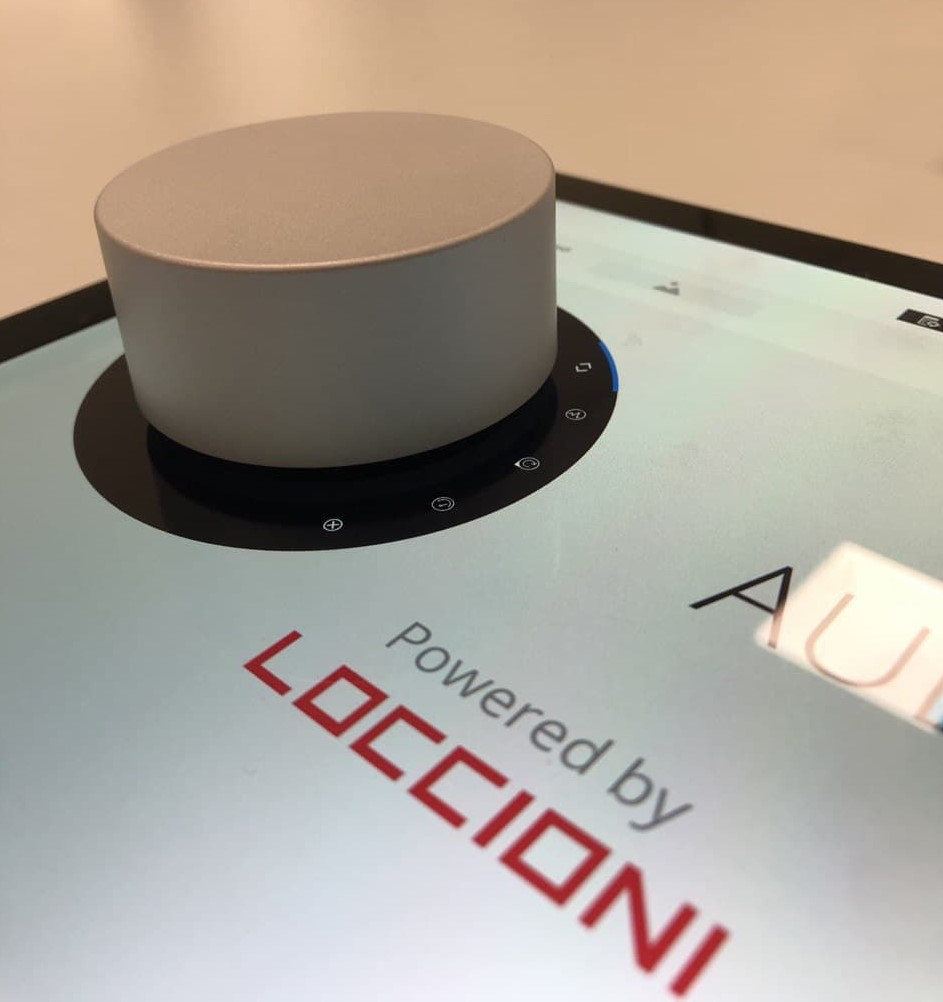
\includegraphics[width=0.5\textwidth]{DialSchermo}
  \caption{Microsoft Dial posizionato sopra un surface pro 6}
\end{figure}
Inizialmente abbiamo preso in considerazione la possibilitá di suddividere il layout dell’applicazione nativa in N riquadri, all’interno dei quali avremo posizionato il relativo Widget da controllare. Questa soluzione presenta peró delle limitazioni, in quanto in base alla risoluzione del dispositivo utilizzato, i widget caricabili in ogni riquadro del layout erano limitati al numero di riquadri definiti dall’applicazione UWP.

Abbiamo quindi cercato una soluzione, che spostasse la responsabilitá di acquisire il posizionamento lato Web anziché lato UWP. Dopo vari tentativi, abbiamo escogitato una soluzione che ci permettesse di avere un numero variabile di Widget configurabili nella Dashboard e la successiva acquisizione di essi, per fare ciò abbiamo sfruttato
Analizzando gli eventi richiamabili dalla classe RadialController, in particolare quelli inerenti al contatto con lo schermo, abbiamo notato prendevano in ingresso un oggetto di tipo RadialControllerScreenContact fornitogli dalla Libreria. Questo oggetto possiede due attributi relativi al Posizionamento ( Position ) e al Bound ( Bounds ) del rettangolo generato dal Dial sullo schermo.

Grazie all’attributo Position di tipo Point, é possibile ottenere, attraverso le coordinate X e Y, il punto centrale nel quale il Dial é posizionato.

\vspace{1.0cm}
\begin{lstlisting}[caption={Metodo ScreenContactStartedAsync},style=javaScriptCode]
 internal async Task ScreenContactStartedAsync(
 	RadialControllerScreenContactStartedEventArgs args
 )
  {
    this.simpleHaptics = args.SimpleHapticsController;
    string x = args.Contact.Position.X.ToString();
    string y = args.Contact.Position.Y.ToString();
    window.PointerPosition = new Point(
    	args.Contact.Position.X, 
    	args.Contact.Position.Y
    	);
    string function = 
    "window.DialFrontendBridge.ScreenContactStartedEvent('" + x + "', '" + y + "')";
    await webView.InvokeScriptAsync("eval", new string[] { function });
    onScreen = true;
    inputInjector.InjectMouseInput(new[] { inputInfo });
    inputInfo.MouseOptions = InjectedInputMouseOptions.Move;
    inputInfo.DeltaY = 1;
  }
\end{lstlisting} 
\vspace{1.0cm}


Attraverso la libreria Window.UI.Core é possibile spostare il cursore in un punto definito della UI corrente. Per questo motivo, la classe WebNotifier presente un attributo private e readonly chiamato window, un oggetto di tipo WindowCore che permette di intercettare eventi relativi ai dispositivi di Input utilizzati ma anche di posizionare il cursore del dispositivo in una posizione specifica in base alle coordinate passategli. In questo modo, attraverso l’attributo PointerPosition siamo stato in grado di creare un nuovo oggetto di tipo Point con le coordinate X e Y acquisite dal Dial consentendoci di posizionare il cursore in quel determinato punto.
\vspace{1.0cm}
\begin{lstlisting}[caption={Spostamento cursore},style=javaScriptCode]
  window.PointerPosition = new Point(args.Contact.Position.X, args.Contact.Position.Y);
\end{lstlisting} 
\vspace{1.0cm}
Questa soluzione ci ha permesso di spostare dinamicamente il cursore nella posizione centrale al disotto del Dial quando viene posizionato sopra lo schermo così da poter intercettare lato Web la posizione del cursore e permettere agli utilizzatori del servizio di riprodurre il comportamente appropriato per il Widget sopra il quale ci si posiziona.
Abbiamo quindi previsto nel Template HTML del Widget un metodo OnMouseOver che venisse richiamato solamente qualora il Dial fosse effettivamente a contatto con lo schermo, ma il semplice spostamento del cursore nella nuova posizione non richiamava correttamente il metodo in quanto il cursore non effettuava un movimento, ma veniva ricreato in quella determinata posizione.
Affinché la soluzione ideata funzionasse correttamente abbiamo importato una libreria chiamata Windows.UI.Input.Preview.Injection che mette a disposizione funziolitá per la simulazione di eventi di input.

Una volta posizionato il cursore nella nuova posizione, siamo stati in grado di simulare un impercettibile movimento del cursore di un singolo pixel, grazie al quale ci é stato possibile intercettare correttamente l’evento OnMouseMove dichiarato nel Template del Widget eseguendo il metodo associato.

\vspace{1.0cm}
\begin{lstlisting}[caption={Spostamento cursore},style=javaScriptCode]
inputInjector.InjectMouseInput(new[] { inputInfo });
inputInfo.MouseOptions = InjectedInputMouseOptions.Move;
inputInfo.DeltaY = 1;
\end{lstlisting} 
\vspace{1.0cm}
